\chapter{Confusion Matrix}
\label{ch:confusion-matrix}\index{confusion matrix|(}

A \textit{Confusion Matrix} (CM), is a contingency table showing how well a model classifies categorical data. By convention \citep{sammut2017encyclopedia}, the CM of an N-class model is an N$\times$N matrix indexed by the true class in the row dimension and the predicted class in the column dimension (Table \ref{tab:cm_spam}).

\begin{table}[ht]
  \centering
  \fontfamily{ppl}\selectfont
  \begin{tabular}{llll}
    \toprule
                        &                     & \multicolumn{2}{c}{\textbf{Predicted Class}} \\
                        &                     & \textit{spam} & \textit{$\neg$spam} \\
    \midrule
    \textbf{True Class} & \textit{spam}       & 10           & 1 \\
                        & \textit{$\neg$spam} & 2            & 100 \\
    \bottomrule
  \end{tabular}
  \caption{CM of a hypothetical binary classifier which predicts whether out-of-sample text objects are spam or not. In this example, 10 spam and 100 non-spam objects are classified correctly, whilst 1 spam and 2 non-spam objects are misclassified.}
  \label{tab:cm_spam}
\end{table}
\vspace{2mm}

Even though CMs are commonly used to evaluate binary classifiers, they are not restricted to 2-class models \citep{martin2018speech}. A CM of a multi-class model would show the number of times the classes were predicted correctly and which classes were confused with each other (Table \ref{tab:cm_sweets}).

\begin{table}[ht]
  \centering
  \fontfamily{ppl}\selectfont
  \begin{tabular}{llll}
    \toprule
                      & \textit{M\&M's} & \textit{Skittles} & \textit{Smarties} \\
    \midrule
    \textit{M\&M's}   & 34              & 3                 & 8  \\
    \textit{Skittles} & 1               & 28                & 5  \\
    \textit{Smarties} & 2               & 4                 & 22 \\
    \bottomrule
  \end{tabular}
  \caption{CM of a hypothetical sweets classifier. The main diagonal of the CM shows the number of correct predictions, whilst the remaining elements indicate how many sweets were misclassified.}
  \label{tab:cm_sweets}
\end{table}
\vspace{2mm}

The CM of the model $h : X \mapsto C$ over the concept $c : X \mapsto C$ using dataset $S \subset X$ is formally defined  as a matrix $\Xi$ such that $\Xi_{c,S}(h)[d_1,d_2] = |S_{h=d_1,c=d_2}|$ \citep{cichosz2014data}. The CM is constructed by incrementing the element corresponding to the true class \textit{vis-a-vis} the predicted class for each object in the dataset (Algorithm \ref{alg:cm}).

\begin{algorithm}
  \begin{algorithmic}
    \State $\Xi \gets 0$
    \For{$x \in S$}
      \State $d_1 \gets c(x)$
      \State $d_2 \gets h(x)$
      \State $\Xi_{d_1,d_2} \gets \Xi_{d_1,d_2} + 1$
    \EndFor
  \end{algorithmic}
  \caption{The CM is initialised to the zero matrix, and populated by iterating over all the objects $x$ with corresponding true class $d_1$ and predicted class $d_2$ and incrementing the element $(d_1,d_2)$ by 1 for each matching outcome.}
  \label{alg:cm}
\end{algorithm}

In binary classification, the CM consists of 2 specially designated classes called the \textit{positive} class and the \textit{negative} class \citep{saito2015precision}. As indicated in Table \ref{tab:cm_binary}, positive outcomes from the true class  which are classified correctly are called \textit{True Positives}\index{true positives} (TP), whilst misclassifications are called \textit{False Negatives}\index{false negatives} (FN). On the other hand, negative true class outcomes which are classified correctly are called \textit{True Negatives}\index{true negatives} (TN), and misclassifications are called \textit{False Positives}\index{false positives} (FP). In natural sciences, FP are called \textit{Type I Errors} and FN are known as \textit{Type II Errors} \citep{fielding1997review}.

\begin{table}[ht]
  \centering
  \fontfamily{ppl}\selectfont
  \begin{tabular}{lll}
    \toprule
                  & \textit{+ve} & \textit{-ve} \\
    \midrule
    \textit{+ve}  & TP           & FN \\
    \textit{-ve}  & FP           & TN \\
    \bottomrule
  \end{tabular}
  \caption{CMs of binary classifiers have positive (+ve) and negative (-ve) classes, and elements called \textit{True Positives} (TP), \textit{False Positives} (FP), \textit{True Negatives} (TN) and \textit{False Negatives} (FN).}
  \label{tab:cm_binary}
\end{table}
\vspace{2mm}

The information presented in the CM can be used to evaluate the performance of different binary classifiers \citep{lu2004predicting}. A number of statistics (Eq. \ref{eq:cm_acc}-\ref{eq:cm_fscore}) derived from the CM have been proposed in the literature \citep{deng2016improved} to gain a better understanding of what are the strengths and weaknesses of different classifiers. Caution should be exercised when interpreting metrics \citep{jeni2013facing}, since the CM could be misleading if the data is imbalanced and an important subrange of the domain is underrepresented \citep{raeder2012learning}. For instance, an albino zebra classifier which always returns negative will achieve high accuracy since albinism is a rare disorder.

These metrics are important in situations in which a particular type of misclassification, i.e. FP or FN, could have worse consequences than the other \citep{hassanien2017advances}. For example, FP are more tolerable than FN in classifiers which predict whether a patient has a disease. Both outcomes are undesirable, but in medical applications it is better to err on the side of caution since FN could be fatal.

\textit{Accuracy}\index{confusion matrix!accuracy} (ACC) is the proportion of correct predictions (Eq. \ref{eq:cm_acc}). It is a class-insensitive metric because it can give a high rating to a model which classifies majority class objects correctly but misclassifies interesting minority class objects \citep{branco2016survey}. The other metrics should be preferred since they are more class-sensitive and give better indicators when the dataset is imbalanced.

\begin{equation}
\label{eq:cm_acc}
ACC = \frac{|TP \cup TN|}{|TP \cup FP \cup TN \cup FN|}
\end{equation}

\textit{Negative Predictive Value}\index{confusion matrix!negative predictive value} (NPV) is the ratio of the correct negative predictions from the total negative predictions (Eq. \ref{eq:cm_npv}).

\begin{equation}
\label{eq:cm_npv}
NPV = \frac{|TN|}{|TN \cup FN|}
\end{equation}

\textit{True Negative Rate}\index{confusion matrix!true negative rate} (TNR), or \textit{Specificity}\index{confusion matrix!true negative rate!specificity}, is the ratio of the correct negative predictions from the total true negatives (Eq. \ref{eq:cm_tnr}).

\begin{equation}
\label{eq:cm_tnr}
TNR = \frac{|TN|}{|TN \cup FP|}
\end{equation}

\textit{True Positive Rate}\index{confusion matrix!true positive rate} (TPR), also called \textit{Sensitivity}\index{confusion matrix!true positive rate!sensitivity} or \textit{Recall}\index{confusion matrix!true positive rate!recall}, is the ratio of the correct positive predictions from the total true positives (Eq.\ref{eq:cm_tpr}).

\begin{equation}
\label{eq:cm_tpr}
TPR = \frac{|TP|}{|TP \cup FN|}
\end{equation}

Sensitivity and Specificity can be combined into a single metric (Eq. \ref{eq:cm_ss}). These metrics are often used in  domains in which minority classes are important \citep{kuhn2013applied}. For example, the Sensitivity of a medical classifier \citep{el2010hybrid} measures how many patients with the condition tested positive, and Specificity measures how many did not have the condition and tested negative.

\begin{equation}
\label{eq:cm_ss}
\textnormal{\textit{Sensitivity}} \times \textnormal{\textit{Specificity}} = \frac{|TP| \times |TN|}{|TP \cup FN| \times |TN \cup FP|}
\end{equation}

\textit{Positive Predictive Value}\index{confusion matrix!positive predictive value} (PPV), or \textit{Precision}\index{confusion matrix!positive predictive value!precision}, is the ratio of the correct positive predictions from the total positive predictions (Eq. \ref{eq:cm_ppv}). The difference between accuracy and precision is depicted in Fig. \ref{fig:cm_accprec}.

\begin{equation}
\label{eq:cm_ppv}
PPV = \frac{|TP|}{|TP \cup FP|}
\end{equation}

\begin{marginfigure}
  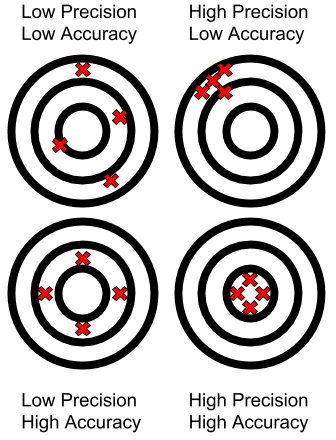
\includegraphics{confusion_matrix/accprec.png}
  \caption{Accuracy vs Precision.}
  \label{fig:cm_accprec}
\end{marginfigure}

Precision and Recall are borrowed from the discipline of \textit{Information Extraction} \citep{sokolova2009systematic}. A composite metric called \textit{F-score}\index{confusion matrix!f-score}, \textit{F1-score}\index{confusion matrix!f-score!f1-score}, or \textit{F-measure}\index{confusion matrix!f-score!f-measure} (Eq. \ref{eq:cm_fscore}) can be derived by finding their harmonic mean \citep{kelleher2015fundamentals}.

\begin{equation}
\label{eq:cm_fscore}
\textnormal{\textit{F-score}} = 2 \times \frac{PPV \times TPR}{PPV + TPR}
\end{equation}

The complements of ACC, NPV, TNR, TPR and PPV are called, respectively, \textit{Error Rate}\index{confusion matrix!error rate}, \textit{False Omission Rate}\index{confusion matrix!false omission rate}, \textit{false positive rate}\index{confusion matrix!false positive rate}, \textit{false negative rate}\index{confusion matrix!false negative rate} and \textit{False Discovery Rate}\index{confusion matrix!false discovery rate}.

The metrics can be adapted for evaluating multi-class models by decomposing an N-class CM into 2-class CMs, and evaluating them individually \citep{stager2006dealing}. The literature describes two methods for decomposing this kind of  CM. In the \textit{1-vs-1}\index{confusion matrix!1-vs-1} approach, 2-class CMs are constructed for each pairwise class as shown in Table \ref{tab:cm_1vs1}.

\begin{table}[ht]
  \centering
  \fontfamily{ppl}\selectfont
  \begin{tabular}{ll}
    \toprule
    \textit{+ve} & \textit{-ve} \\
    \midrule
    M\&M's       & $\{$Skittles, Smarties$\}$ \\
    Skittles     & $\{$M\&M's, Smarties$\}$ \\
    Smarties     & $\{$M\&M's, Skittles$\}$ \\
    \bottomrule
  \end{tabular}
  \caption{2-class CMs derived from the classes in Table \ref{tab:cm_sweets}. The +ve classes are paired separately with each -ve class.}
  \label{tab:cm_1vs1}
\end{table}
\vspace{2mm}

In the \textit{1-vs-rest}\index{confusion matrix!1-vs-rest} approach, 2-class CMs are constructed for each class and the remaining classes combined together as shown in Table \ref{tab:cm_1vsN}.

\begin{table}[ht]
  \centering
  \fontfamily{ppl}\selectfont
  \begin{tabular}{ll}
    \toprule
    +ve       & -ve \\
    \midrule
    M\&M's    & Skittles $\cup$ Smarties \\
    Skittles  & M\&M's $\cup$ Smarties \\
    Smarties  & Skittles $\cup$ M\&M's \\
    \bottomrule
  \end{tabular}
  \caption{2-class CMs derived through decomposition of the 3-class CM from Table \ref{tab:cm_sweets} using the 1-vs-rest approach.}
  \label{tab:cm_1vsN}
\end{table}
\vspace{2mm}

Using all metrics could be counterproductive due to information redundancy, but none of the metrics is enough on its own \citep{ma2007adequate}. For instance, Recall is class-sensitive but it would give a perfect score to an inept model which simply returns the positive class. Thus, the best approach is to evaluate with complementary pairs \citep{gu2009evaluation} such as Sensitivity \textit{vs} Specificity, or Precision \textit{vs} Recall; or a combined measure such as the F-score.

Taking into account the above, CMs are suitable for visualising, evaluating, and comparing the performance of binary or multi-class classifiers. They should be used in conjunction with metrics such as the F-measure to avoid bias, especially if the dataset is unbalanced. For further details on the theoretical aspects of CMs and for practical examples in R refer to \citep{cichosz2014data}; for examples in Python refer to \citep{muller2016introduction}.

The following example is motivated by the samples in the \textit{Scikit-Learn} documentation and the work of  \citep{geron2017hands}. The models in Fig. \ref{fig:cm_model} were trained on the \textit{wines} dataset included with Scikit-Learn.

\begin{figure}
  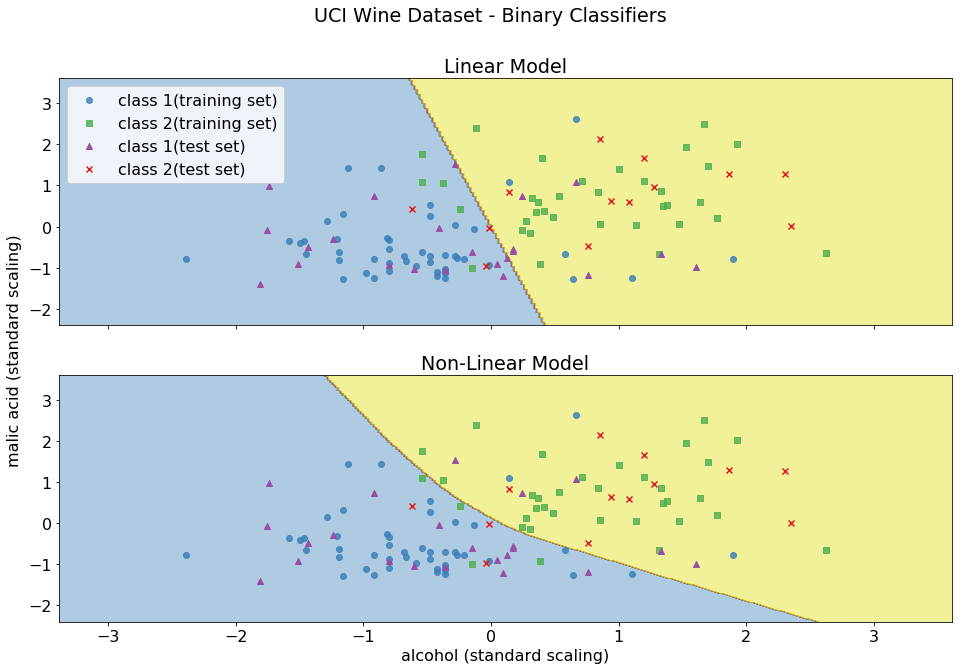
\includegraphics{confusion_matrix/model.png}
  \caption{Decision boundary learned by a linear and non-linear binary classifier.}
  \label{fig:cm_model}
\end{figure}

\begin{margintable}
  \begin{tabular}{lll}
    \toprule
                 & Linear & Non-Linear \\
    \midrule
    Accuracy     & 0.72   & 0.78 \\
    Specificity  & 0.77   & 0.77 \\
    Sensitivity  & 0.70   & 0.78 \\
    Precision    & 0.84   & 0.86 \\
    F-score      & 0.76   & 0.82 \\
    \bottomrule
  \end{tabular}
  \caption{Statistics derived from the CMs in Fig. \ref{fig:cm_wines}.}
  \label{tab:cm_metrics}
\end{margintable}

As it can be intuitively deduced from Fig. \ref{fig:cm_model}, the decision boundary of the non-linear model is a better fit than the linear model. The CMs in Fig. \ref{fig:cm_wines} also show that non-linear model performs better with a higher TP, and consequently lower TN. The biggest advantage of the non-linear model is the higher Sensitivity resulting in a better F-score.

\begin{figure}
  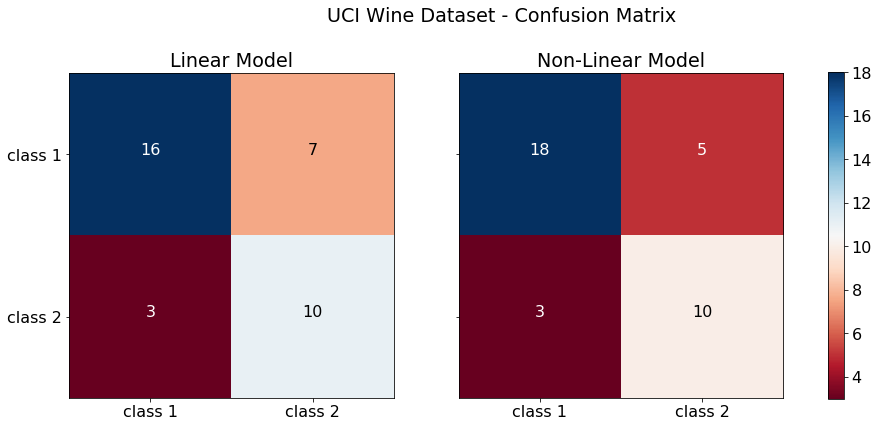
\includegraphics{confusion_matrix/cm.png}
  \caption{The linear classifier has 16 TP, 10 TN, 7 FN and 3 FP, whilst the non-linear classifier has 18 TP, 10 TN, 5 FN and 3 FP.}
  \label{fig:cm_wines}
\end{figure}

\index{confusion matrix|)}